\section{Results}
% Provide an introductory paragraph that summarizes what's in this section: a list of runs/experiments intended to test your implementation and ideas. Describe each of these experiments in a few words/a sentence.

This section presents the results of our experiments evaluating various matrix-vector multiplication (VMM) methods. We conducted a series of experiments to measure and compare the computational throughput, memory bandwidth utilization, and speedup of different VMM implementations, including VMM Basic, VMM Vectorized, VMM CBLAS, and VMM OpenMP. The goal was to understand the performance benefits and limitations of various parallelization techniques.

\subsection{Computational platform and Software Environment}
\label{sec:computational-platform-and-software-environment}

% The experiments were conducted on the CPU node of the Perlmutter supercomputer at NERSC. Each CPU node is equipped with two AMD EPYC 7763 (Milan) processors, each with 64 cores running at a clock rate of 2.45 GHz \cite{nersc_perlmutter_architecture}. Each core is equipped with 32 KB of L1 cache and 512 KB of L2 cache, while 8 cores share a 32 MB L3 cache \cite{amd_epyc_tuning_guide}. The system is supported by 512 GB of DDR4 DRAM, providing a memory bandwidth of 204.8 GB/s per CPU \cite{nersc_perlmutter_architecture}. The processor utilizes the AVX2 instruction set for vector processing, and each core offers a peak computational throughput of 39.2 GFLOPS \cite{nersc_perlmutter_architecture}.
The experiments were conducted on the CPU node of the Perlmutter supercomputer at NERSC. Each CPU node is equipped with two AMD EPYC 7763 (Milan) processors, each with 64 cores running at a clock rate of 2.45 GHz. Each core supports Simultaneous Multi-threading (SMT), which allows 2 threads per core to run simultaneously when enabled. Each core is equipped with 32 KB of L1 cache and 512 KB of L2 cache, while 8 cores share a 32 MB L3 cache. Each AMD EPYC 7763 (Milan) processor contains 8 memory channels per socket, 2 DIMMs per memory channel, and has 4 NUMA domains per socket (NPS=4) \cite{amd_epyc_tuning_guide}.

The system is supported by 512 GB of DDR4 DRAM, providing a memory bandwidth of 204.8 GB/s per CPU. The processor utilizes the AVX2 instruction set for vector processing, and each core offers a peak computational throughput of 39.2 GFLOPS \cite{nersc_perlmutter_architecture}.


All experiments were performed on a single CPU node running \textit{SUSE Linux Enterprise Server 15 SP4}, with kernel version \textit{5.14.21-150400.24.81\_12.0.87-cray\_shasta\_c} \cite{usami2024hostnamectl}. The C++ code was compiled using \textit{g++-12 (SUSE Linux) 12.3.0} with the following optimization flags for each implementation:

\begin{itemize}
    \raggedright    
    \item \textbf{VMM Basic (Serial)}: Compiled with \texttt{-march=native -O1} for basic optimizations without vectorization or parallelization, ensuring native architecture optimizations.

    \item \textbf{VMM Vectorized (Serial)}: Compiled with \texttt{-O3 -DNDEBUG -fomit-frame-pointer -ftree-vectorize -funroll-loops -ffast-math -fopt-info-vec-all=report.txt}. These flags enable vectorization, loop unrolling, and fast math optimizations to achieve higher performance through vectorized operations.
    
    \item \textbf{VMM OpenMP (Parallel)}: Compiled with \texttt{-fopenmp -march=native -O1} to enable OpenMP parallelization in multiple threads. The \texttt{-march=native} flag ensures optimization for the native architecture, while \texttt{-O1} is used for moderate optimization, avoiding overly aggressive optimizations that might conflict with parallelization.
    
    \item \textbf{VMM CBLAS}: Compiled with \texttt{-march=native -O0} to ensure native architecture optimization without further compiler optimizations, relying on the performance of the CBLAS library itself.
\end{itemize}

The following OpenMP environmental variables were used when running VMM OpenMP, with \texttt{OMP\_NUM\_THREADS} set according to the number of threads:
\begin{itemize}
    \item \texttt{OMP\_PLACES=threads}: This variable specifies how OpenMP should assign threads to processing units. Setting it to \texttt{threads} ensures that each OpenMP thread is assigned to a separate hardware thread.
    
    \item \texttt{OMP\_PROC\_BIND=spread}: This variable controls how threads are bound to processors. Setting it to 	\texttt{spread} aims to distribute threads as evenly as possible across the available CPUs.
    
    \item \texttt{OMP\_SCHEDULE=static} (default): This variable controls how iterations of a parallel loop are divided among threads. The \texttt{static} schedule assigns chunks of iterations to threads in a predetermined manner.
\end{itemize}
% What machine did you run your tests on? What was the processor, its clock rate (GHz), size of L1/L2/L3 cache, how much memory (DRAM), what OS?

% What compiler did you use, what compilation flags?

\subsection{Methodology}
\label{sec:methodology}
% Describe the procedures you use to test your system.
We evaluated the performance of various matrix-vector multiplication (VMM) methods using matrix sizes of \(1024 \times 1024\), \(2048 \times 2048\), \(4096 \times 4096\), \(8192 \times 8192\), and \(16384 \times 16384\). For the VMM OpenMP (Parallel) implementation, we tested with thread counts of 1, 4, 16, and 64. 

To avoid skewed results caused by the known issue of slow performance during the first run of VMM CBLAS (due to dynamic library loading), we first performed a warm-up run using the \(1024 \times 1024\) matrix size. This initial run was discarded to ensure that subsequent performance measurements were representative. 

Performance was measured by calculating the elapsed time using instrumentation placed around the core matrix-vector multiplication code, as shown in Listing~\ref{listing:measuring-elapsed-time}. Based on the elapsed time, we derived three key performance metrics: 
\begin{itemize}
    \item Computational Throughput
    \item Memory Bandwidth Utilization
    \item Speedup at varying levels of concurrency for the VMM OpenMP (Parallel) implementation.
\end{itemize}

\begin{lstlisting}[caption={Instrumentation code for measuring the elapsed time of matrix-vector multiplication},label={listing:measuring-elapsed-time},name=measuring-elapsed-time,float=htbp,style=mystyle,language=C++]
setup(n, A, X, Y);
start_time = get_high_resolution_clock_now();
my_dgemv(n, A, X, Y);
end_time = get_high_resolution_clock_now();
elapsed_time = end_time - start_time;
\end{lstlisting}

\subsubsection{Computational Throughput}
\label{subsubsec:mflops}

\begin{displaymath}
    MFLOP/s = \frac{\textit{ops}}{\textit{runtime} \times 10^6}
\end{displaymath}
\begin{displaymath}
    GFLOP/s = \frac{\textit{ops}}{\textit{runtime} \times 10^9} 
\end{displaymath}
\begin{displaymath}
    \textit{ops} = 2N^2
\end{displaymath}

Here, \textit{ops} represents the number of floating-point operations required to multiply \(N \times N\) matrix and \(N\) size vector \footnote{When the matrix size is \(N \times N\), the number of floating-point operations (FLOPs) required for matrix-vector multiplication (VMM) is approximately \(2N^2\). This is because matrix-vector multiplication involves \(N\) dot products, each requiring \(2N\) operations (one multiplication and one addition per element).}. The \textit{runtime} is the time elapsed (in seconds) measured for each matrix multiplication method and size.


\subsubsection{Memory Bandwidth Utilization}
\label{subsubsec:memory-bandwidth-utilization}

\begin{displaymath}
    \text{Memory Bandwidth Utilization (\%)} = \frac{\textit{bytes}}{\textit{runtime} \times \textit{capacity}}
\end{displaymath}
\begin{displaymath}
    \textit{bytes} = \frac{(2N + 2N^2) \times 8}{10^9}
\end{displaymath}
\begin{displaymath}
    \textit{capacity} = 204.8 \text{ GB/s} \times 2
\end{displaymath}

Here, \textit{bytes} represents the number of memory bytes accessed to multiply an \(N \times N\) matrix and an \(N\)-size vector, divided by one billion to convert to gigabytes. The \textit{capacity} is the theoretical peak memory bandwidth in gigabytes per second (see Sec.~\ref{sec:computational-platform-and-software-environment}).\footnote{For the matrix-vector multiplication, memory accesses are composed of accessing each element of Y twice (read and write), accessing all elements of A once (read-only), and accessing all elements of X once (read-only), leading to the formula \(2N + 2N^2\).}

\subsubsection{Speedup}
\label{subsubsec:speedup}
We define speedup as the ratio of a parallel program's speed to a sequential program's speed. For a problem size \(n\) and \(p\) parallel ranks (where rank refers to the number of parallel processing units used):

\begin{displaymath}
    S(n, p) = \frac{T^*(n)}{T(n, p)}
\end{displaymath}

Here, \(T^*(n)\) is the time taken by the best serial algorithm on a problem of size \(n\), which in our case is the VMM Vectorized implementation, and \(T(n, p)\) is the time taken to run the program on a problem of size \(n\) using \(p\) parallel ranks.

\subsection{Comparison of VMM CBLAS with VMM Basic and VMM Vectorized}
\label{subsec:comparison-serial}
% Performance metrics: describe exactly what metrics you employ to measure performance. It might be elapsed time from instrumentation code you added around the main computational code. Later in the term, it may be something else.

% Experimental design: did you run tests over a set of prescribed problem sizes? If so, what were they?

\begin{comment}
    \item Chart #1: MFLOPS. Produce a MFLOP/s chart comparing the performance of these three implementations across all problem sizes. The horizontal axis is problem size, the vertical axis is MFLOP/s (which you'll have to derive from runtime and your knowledge of the algorithm).
    \item Discuss the performance of your Basic VMM and Vectorized VMM across the set of problem sizes. Do you see any changes of MFLOP/s across problem sizes? Describe the nature of those changes, if any, and provide an explanation of why the performance numbers change.
    \item How does the performance of your Basic VMM and Vectorized VMM implementations compare to CBLAS, the reference implementation? Why do you think that is the case? Couch your answers in terms of how the codes make use of the memory subsystem, instruction-level parallelism, and so forth.
\end{comment}

In this experiment, the objective is to establish a baseline for evaluating the computational throughput (MFLOP/s) of three different VMM implementations: VMM Basic (without vectorization or parallelization), VMM Vectorized (automatically vectorized by the compiler), and VMM CBLAS (a highly optimized serial implementation). All three implementations are serial, providing a foundation for comparison against the OpenMP parallel implementation that will be evaluated later. The configuration details for this experiment are provided in Sec.~\ref{sec:methodology}.

\subsubsection{Performance of VMM Basic and VMM Vectorized}
\label{subsubsec:comparison-basic-vectorized}
As shown in Figure~\ref{fig:mflops-serial}, the VMM Vectorized implementation consistently outperforms VMM Basic across all problem sizes. The MFLOP/s of the VMM Basic implementation is relatively stable, averaging around 2300 MFLOP/s. For the VMM Vectorized implementation, the performance peaks at \(N = 1K)\footnote{In this paper, K notation for vector and matrix sizes represents 1024 elements rather than the conventional 1000.}\) with 9986.4 MFLOP/s and decreases slightly to 9118.1 MFLOP/s at \(N = 2K\). For larger problem sizes (\(N = 4K\) to \(N = 16K\)), the performance stabilizes around 8000 MFLOP/s.

The superior performance of the VMM Vectorized implementation for \(N = 1K\) and \(N = 2K\) can be attributed to the efficient utilization of the L1 cache. Specifically, as shown in Table~\ref{tab:memory-footprint-two-vectors}, the combined memory footprint of \(A[i]\) and vector \(x\) (comprising \(2N\) double elements) fits within the L1 cache for these problem sizes. This ensures that vector \(x\) is not evicted from the L1 cache, as both \(A[i]\) and \(x\) are accessed in each iteration of the outer loop.

For problem sizes ranging from \(N = 4K\) to \(N = 16K\), the performance of the VMM Vectorized implementation remains relatively stable because, while the vectors no longer fit in the L1 cache, they do fit in the L2 cache across all these problem sizes, as indicated in Table~\ref{tab:memory-footprint-two-vectors}.

\begin{figure}[htbp]
    \centering
    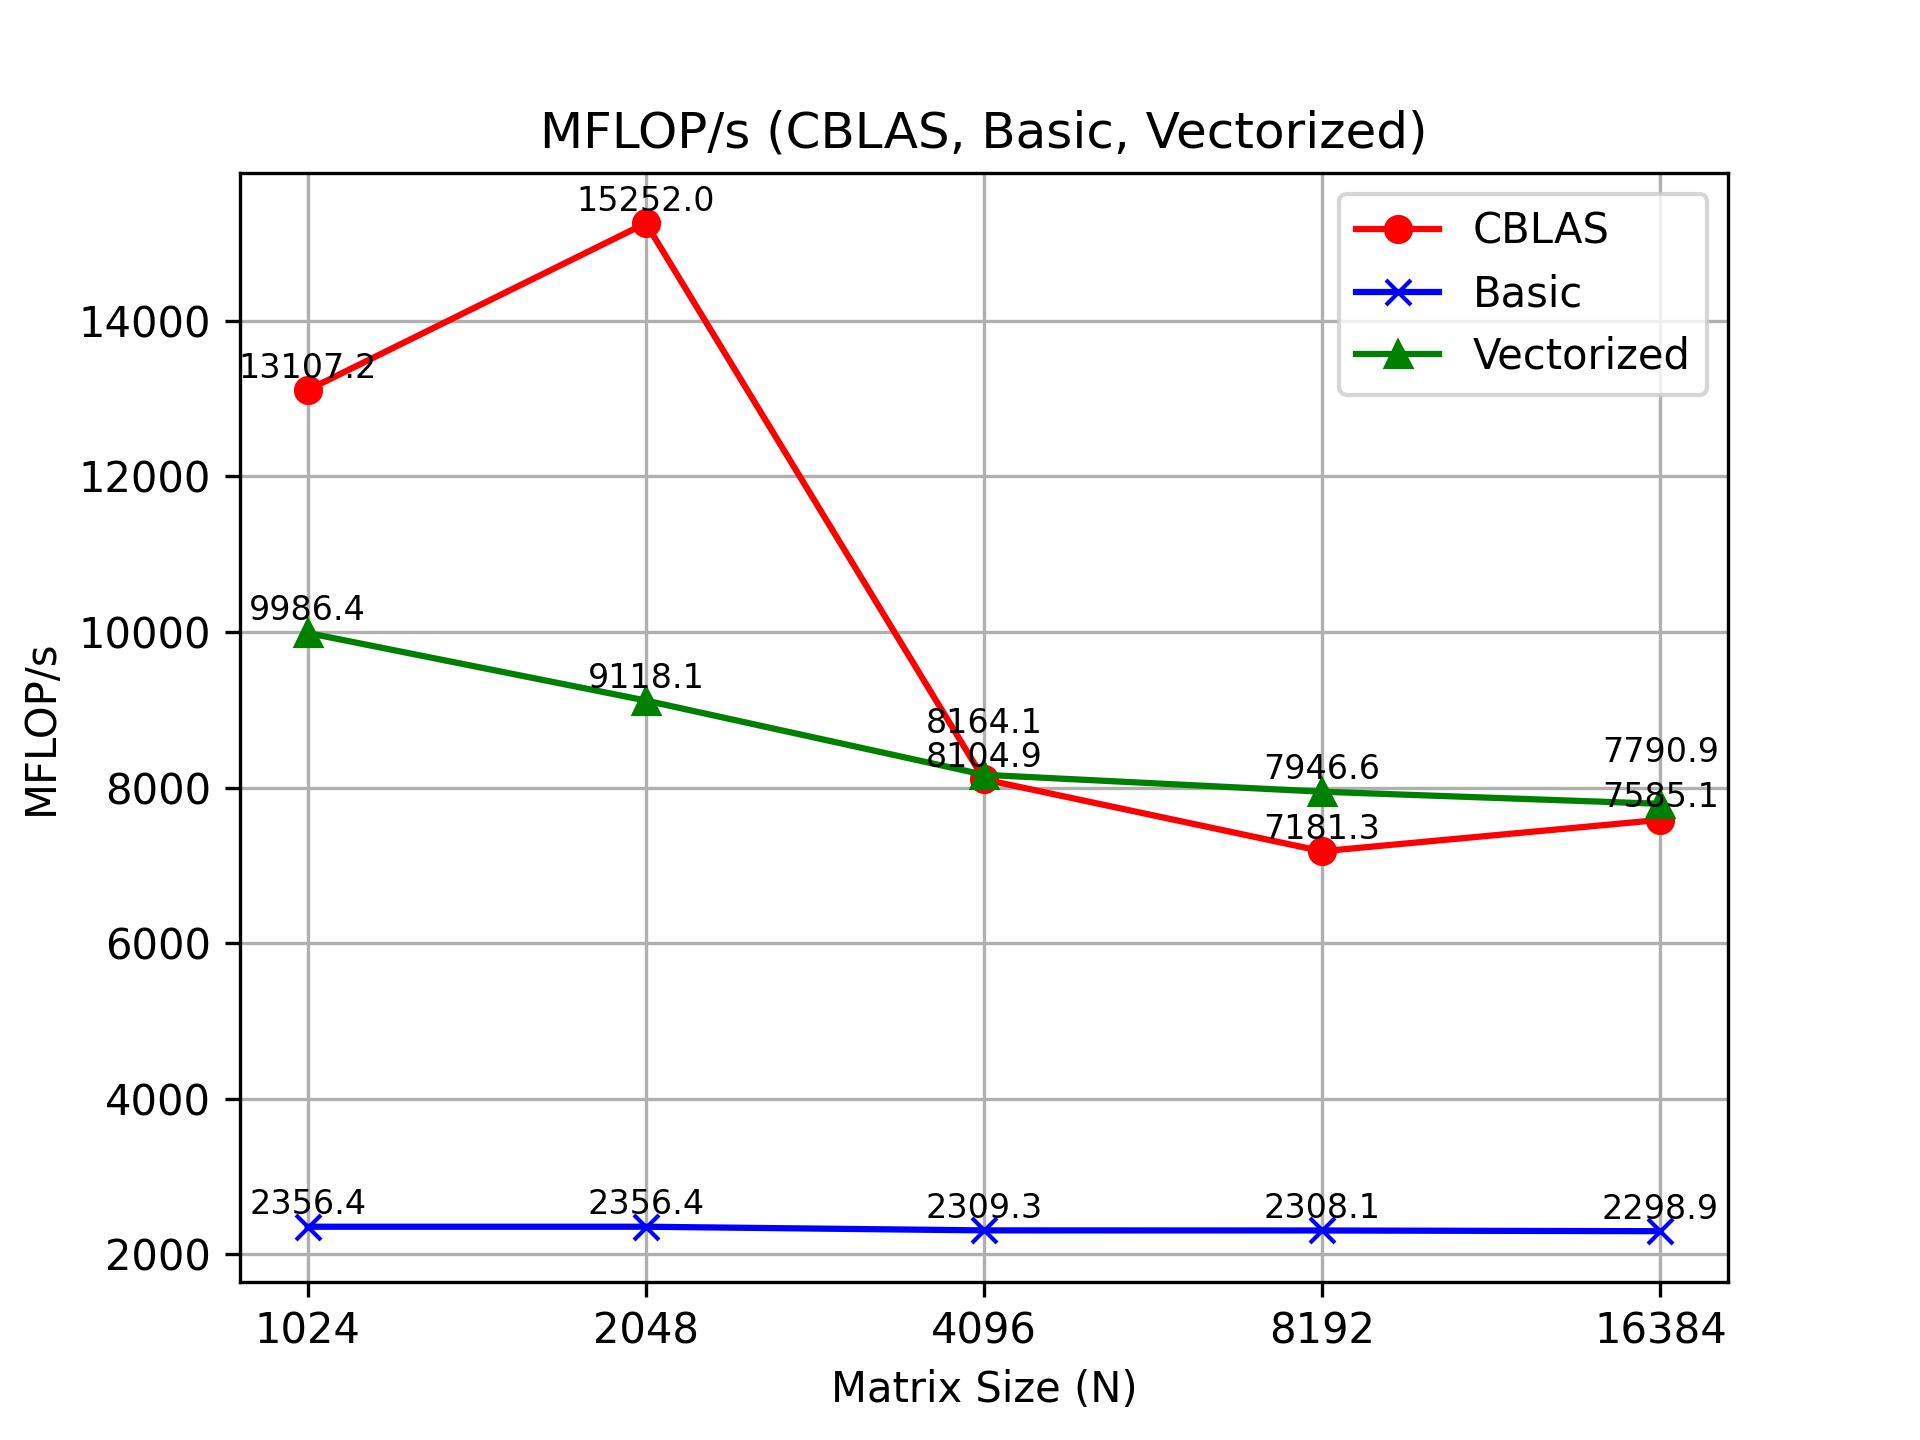
\includegraphics[width=1.0\linewidth]{images/MFLOPs-serial.png}
    \caption{\textbf{MFLOP/s Comparison of VMM CBLAS with VMM Basic and VMM Vectorized across different matrix sizes.} The figure illustrates the computational throughput (MFLOP/s) for each implementation across varying matrix sizes, highlighting the relative performance differences between VMM Basic, VMM Vectorized, and VMM CBLAS. VMM CBLAS demonstrates superior performance for smaller matrix sizes due to efficient cache utilization, while VMM Vectorized shows competitive performance at larger sizes by leveraging automatic vectorization. VMM Basic remains stable but underperforms compared to the other two implementations due to the lack of SIMD utilization and other optimizations.}
    \label{fig:mflops-serial}
\end{figure}

\begin{table}[htbp]
    \centering
    \begin{tabular}{c|c|c|c}
        \textbf{Vector Size (K=1024)} & \textbf{2 Vector (Bytes)} & \textbf{L1} & \textbf{L2} \\
        \hline
        \(1K\) & 16 KiB& Yes & Yes\\
        \(2K\)  & 32 KiB& Yes & Yes\\
        \(4K\)  & 64 KiB& No & Yes\\
        \(8K\)  & 128 KiB& No & Yes\\
        \(16K\)  & 256 KiB& No & Yes\\
    \end{tabular}
    \caption{\textbf{Memory footprint for different vector sizes and L1/L2 cache fit.} The table shows the memory required for two vectors of each size and whether they fit within the L1 cache (32 KiB) and L2 cache (256 KiB). Vector sizes up to \(2K\) fit in L1, while \(4K\) does not.}
    \label{tab:memory-footprint-two-vectors}
\end{table}

\subsubsection{Comparison of VMM CBLAS and VMM Vectorized}
\label{subsubsec:comparison-cblas-vectorized}
The VMM CBLAS implementation consistently outperforms VMM Basic but shows varying results compared to VMM Vectorized depending on the problem size. For smaller problem sizes (\(N = 1K\) and \(N = 2K\)), VMM CBLAS significantly outperforms VMM Vectorized by approximately 30\% and 70\%, respectively. However, for larger problem sizes (\(N = 4K\), \(N = 8K\), and \(N = 16K\)), VMM Vectorized slightly outperforms VMM CBLAS.

The AMD EPYC 7763 processor, which utilizes the AVX2 instruction set (see Sec.~\ref{sec:computational-platform-and-software-environment}), supports 256-bit SIMD instructions. This enables four arithmetic operations on double-precision (64-bit) data in a single cycle, explaining the approximately 400\% performance improvement observed for both VMM CBLAS and VMM Vectorized compared to VMM Basic for larger matrix sizes.

However, the observed performance differences indicate that VMM CBLAS is significantly better optimized for cache utilization under these conditions. For smaller values of \(N\), the performance of CBLAS is 6 to 8 times better than that of VMM Basic, which is a surprising result that cannot be fully explained by SIMD utilization alone. As shown in Table~\ref{tab:memory-footprint-matrices}, for matrix sizes \(N = 1K\) and \(N = 2K\), the matrices fit within the L3 cache, suggesting more efficient cache usage by CBLAS for these sizes. Given that each element of matrix \(A\) is accessed only once during the matrix-vector multiplication, spatial locality does not appear to be a limiting factor. Additionally, since both \(x\) and \(A[i]\) fit in the L1 cache for these sizes, temporal locality also does not seem to be a limiting factor. It is likely that CBLAS achieves superior performance through advanced optimizations such as efficient instruction scheduling, prefetching, and effective exploitation of instruction-level parallelism (ILP), which allows multiple instructions to be executed simultaneously by overlapping their execution stages. CBLAS likely leverages ILP by replicating internal components to process multiple instructions concurrently within each pipeline stage.

\begin{table}[htbp]
    \centering
    \begin{tabular}{c|c|c}
        \textbf{Matrix Size (K=1024)} & \textbf{Matrix size (Bytes)} & \textbf{L3} \\
        \hline
        \(1K \times 1K\) & 8 MiB& Yes\\
        \(2K \times 2K\)  & 32 MiB& Yes\\
        \(4K \times 4K\)  & 128 MiB& No \\
        \(8K \times 8K\)  & 512 MiB& No \\
        \(16K \times 16K\)  & 2 GiB& No \\
    \end{tabular}
    \caption{\textbf{Memory footprint for different matrix sizes and L3 cache fit.} The table shows the memory required for matrices of each size and whether they fit within the L3 cache (32 MiB). Matrix sizes up to \(2K \times 2K\) fit in L3, while \(4K \times 4K\) does not.}
    \label{tab:memory-footprint-matrices}
\end{table}

\subsection{Evaluation of VMM OpenMP (Parallel)}
\label{subsec:evaluation-openmp-parallel}
\begin{comment}
    \item Chart \#2: Speedup chart. Run your OpenMP-parallel code using static thread scheduling at varying concurrency [1, 4, 16, 64] across all problem sizes. Create a single chart showing speedup at varying levels of concurrency. Note: this one chart has 4 datasets. In this chart, the horizontal axis is problem size, and the vertical axis is speedup, which will be a number between 1 and P, where P is the maximum concurrency level (in this case, it is 64).
    \item Discuss the features you see in that 4-variable speedup chart using static thread scheduling. What trends and features do you see? Why do you think those are happening?
\end{comment}

Figure~\ref{fig:openmp-parallel-speedup} shows that the speedup for omp-1 is approximately 0.9, which is slightly worse than the best serial implementation across different matrix sizes. This is likely due to some overhead introduced by the OpenMP threading code, even when only one thread is used.

For larger thread counts, the speedup is only between 0.3 to 0.5 for smaller matrix sizes (N=1K, 2K). This can be attributed to the overhead of creating and joining threads, which becomes relatively significant compared to the gain in parallel computation for smaller problems.

For larger matrix sizes (N=4K, 8K, 16K), the speedup achieved by omp-4, omp-16, and omp-64 is relatively stable, ranging between 1.2 to 1.3. Among these, omp-16 shows slightly better performance for larger matrix sizes. This indicates that although some speedup is achieved, it falls far short of the ideal values due to other limiting factors.

We expected to observe a speedup close to 4x for omp-4, 16x for omp-16, and 64x for omp-64, especially for larger matrix sizes, where the overhead of the serial portion and the introduction of multithreading should be minimal according to Amdahl's law\cite{amdahl1967validity}\footnote{Amdahl's law describes the theoretical maximum speedup that can be achieved in a parallel system based on the portion of a task that must be executed serially. The theoretical speedup limit for a problem size \(n\) and \(p\) parallel processors is given by: \( S(n, p) = \frac{1}{f + \frac{1-f}{p}} \), where \(f\) is the portion of the program that must remain serial, and \((1-f)\) is the parallelizable portion. For smaller values of \(f\), the closer the speedup is to the ideal scaling with \(p\).}. However, the observed results fall significantly short of these expectations, indicating unexpected and undesirable bottlenecks in the parallel execution.

The unexpectedly poor performance is due to a bottleneck not in the arithmetic computations but in other components, such as memory bandwidth. We did not allocate the memory across the NUMA nodes when setting up the matrices and vectors, which means the matrix/vector data likely reside entirely within one NUMA node. Each NUMA node has 64 GB of memory, and the total system memory is 512 GB, which is sufficient to hold all the elements for our problem sizes. As a result, even though the program is multithreaded, the available memory bandwidth is constrained, limiting overall performance. This can explain why omp-16 performs slightly better than omp-64; since the bottleneck is not resolvable by adding more threads, increasing the number of threads only introduces additional overhead without yielding further performance gains.

\begin{figure}[htbp]
    \centering
    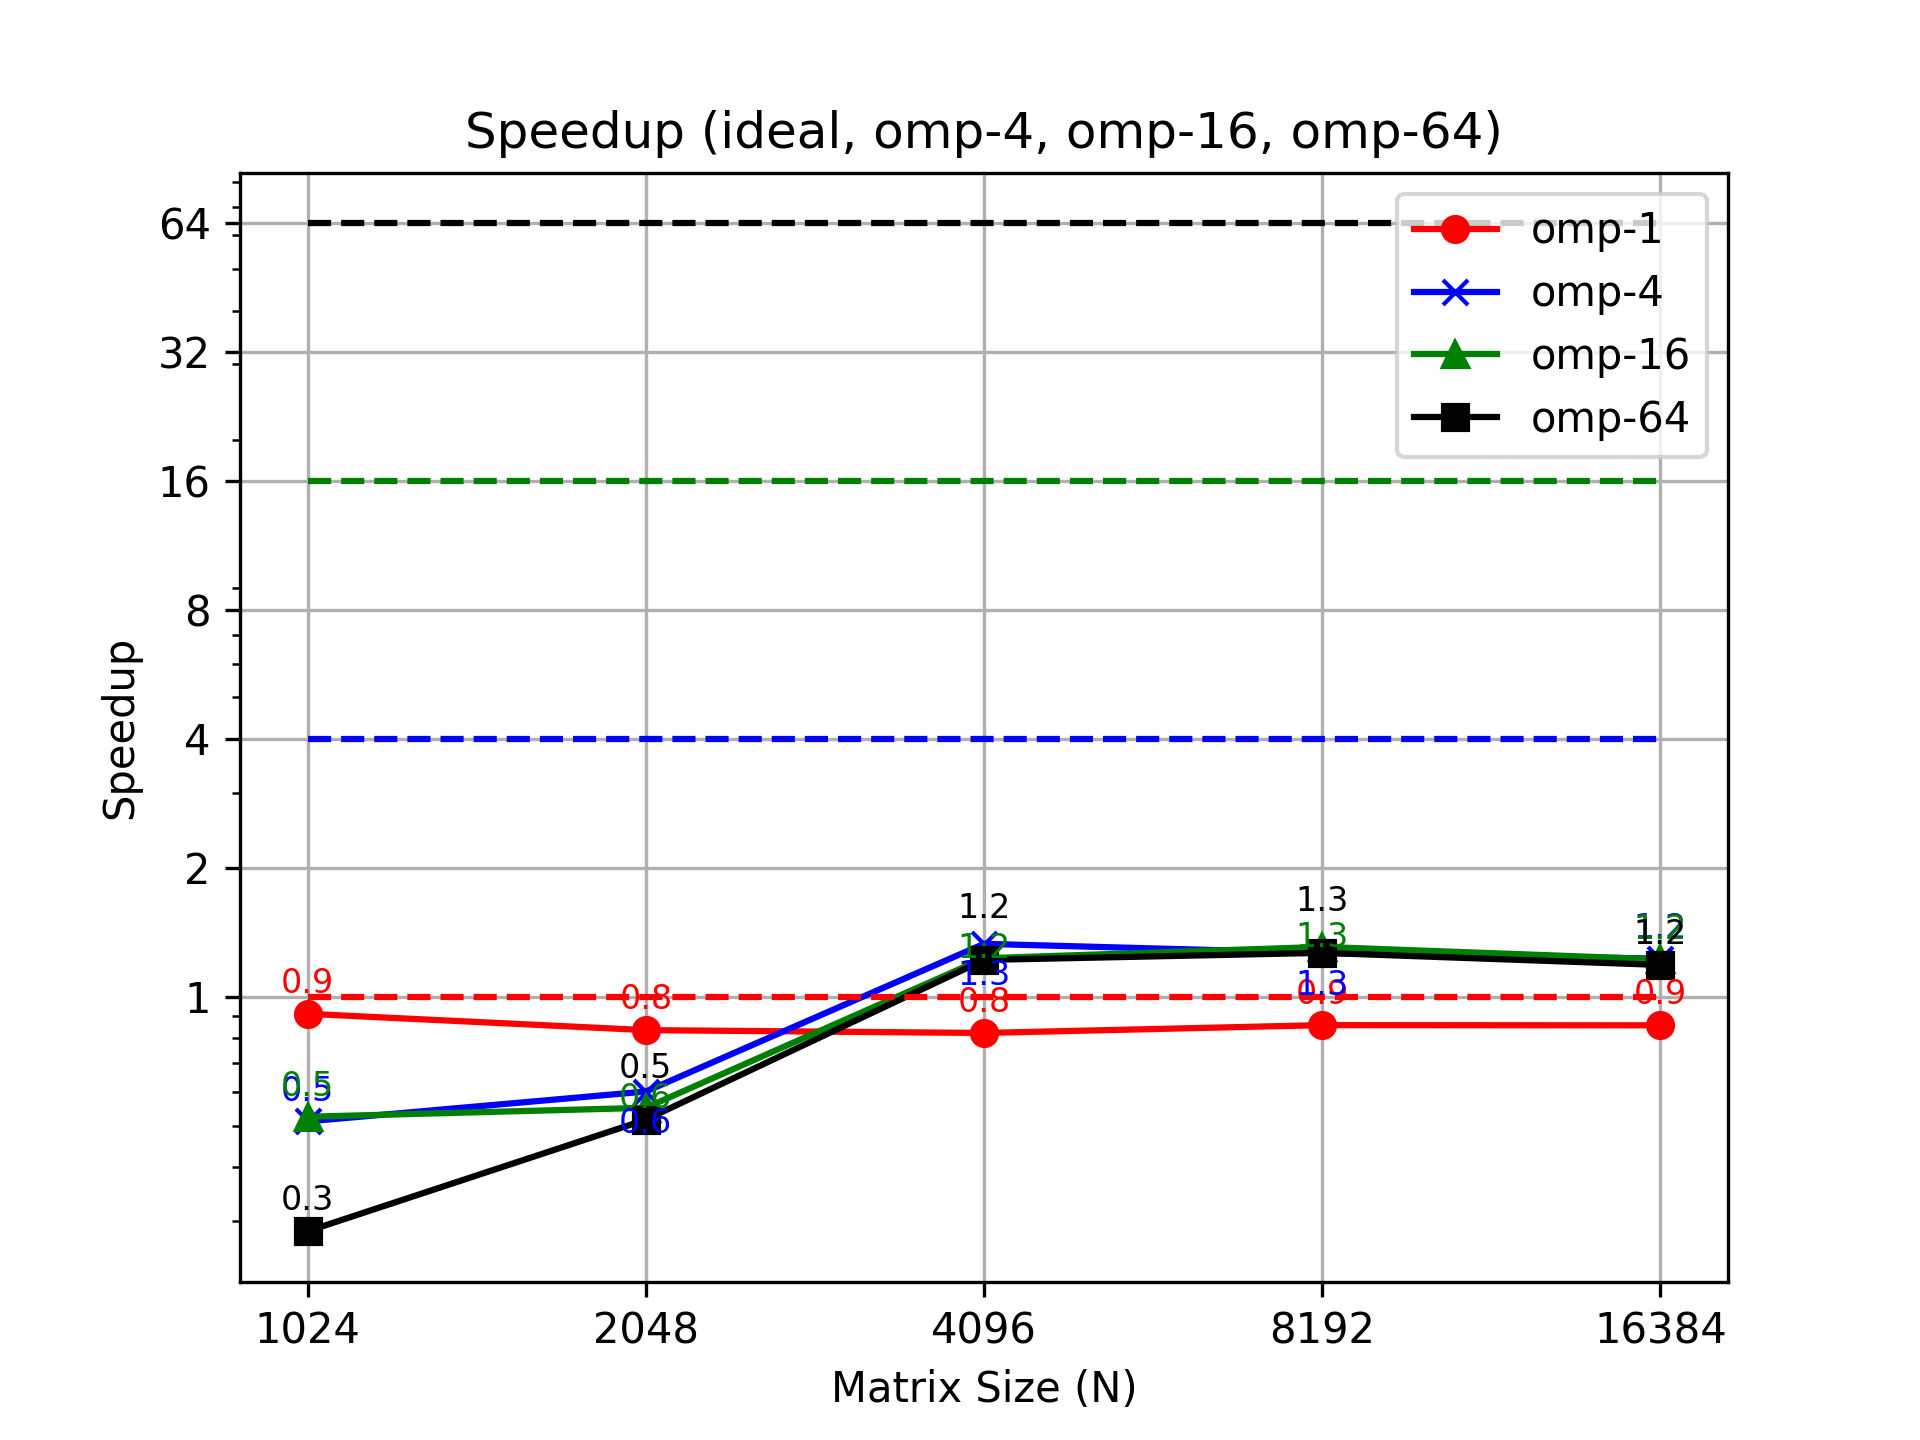
\includegraphics[width=1.0\linewidth]{images/Speedup.png}
    \caption{\textbf{Speedup comparison of OpenMP parallel VMM across different matrix sizes and thread counts.} The figure shows the speedup achieved with different numbers of threads (1, 4, 16, 64) across various matrix sizes. The figure shows that omp-1 performs slightly worse than the best serial implementation due to threading overhead. For smaller matrix sizes, higher thread counts achieve limited speedup due to significant overhead in thread management. For larger matrix sizes, speedup stabilizes around 1.2 to 1.3, indicating bottlenecks in memory bandwidth.}
    \label{fig:openmp-parallel-speedup}
\end{figure}

\subsection{Comparison of VMM OpenMP with VMM CBLAS}
\label{subsec:comparison-openmp-cblas}
% \begin{itemize}
%     \item Chart \#3: MFLOPS. From the previous subsection, identify the the OpenMP Parallel VMM configuration (e.g, which concurrency) that performs the best, and create a 2-variable chart (problem size vs. runtime in MFLOP/s) comparing the MFLOP/s of your best OpenMP configuration with that of a serial CBLAS. In this chart, the horizontal axis is problem size and the vertical axis is MFLOP/s.
%     \item What trends and features do you see in the chart? Why do you think those are happening?
% \end{itemize}

From Figure~\ref{fig:gflops-parallel}, we observed distinct performance differences between the two implementations based on the matrix sizes. For smaller matrix sizes (N=1K and 2K), CBLAS significantly outperformed the OpenMP implementation with 16 threads (omp-16), achieving performance gains of 2.5x to 3.0x. This indicates that CBLAS is better optimized for smaller matrices, where efficient cache use boosts performance, and multi-threading overhead is more significant compared to the performance gain.

For larger matrix sizes (N=4K, 8K, and 16K), omp-16 outperformed CBLAS by 1.2x to 1.4x. As matrix sizes grow beyond the L3 cache capacity, the parallelism advantage in omp-16 becomes more pronounced, surpassing the serial CBLAS implementation. As shown in Table~\ref{tab:memory-footprint-matrices} and Table~\ref{tab:memory-footprint-two-vectors}, when the matrix fits within the L3 cache and both vectors fit in the L1 cache, CBLAS outperforms omp-16, implying more efficient cache use by CBLAS.

Another important factor is the NUMA architecture of the system. Each CPU node has 8 NUMA nodes, with 2 memory channels per NUMA node (see Sec.~\ref{sec:computational-platform-and-software-environment}). Multi-threading can utilize both memory channels in the NUMA node where the data resides, whereas a single-threaded program, like CBLAS, can only utilize a single memory channel. However, the overhead introduced by distributing the threads across NUMA nodes can be significant, approximately doubling the memory access time. This overhead is partly countered by the increased memory bandwidth available to multiple threads\footnote{In the same NUMA node, the memory distance is 10, while the distance for other NUMA nodes in the same CPU is 12, and the distance for NUMA nodes in the other CPU is 32\cite{usami2024numactl}. Therefore, the expected average memory distance when data resides in a single node and threads are scattered is (10 + 12*3 + 32*4)/8 = 21.75, whereas for a single thread in a single memory node, the distance is 10.}.

\begin{figure}[htbp]
    \centering
    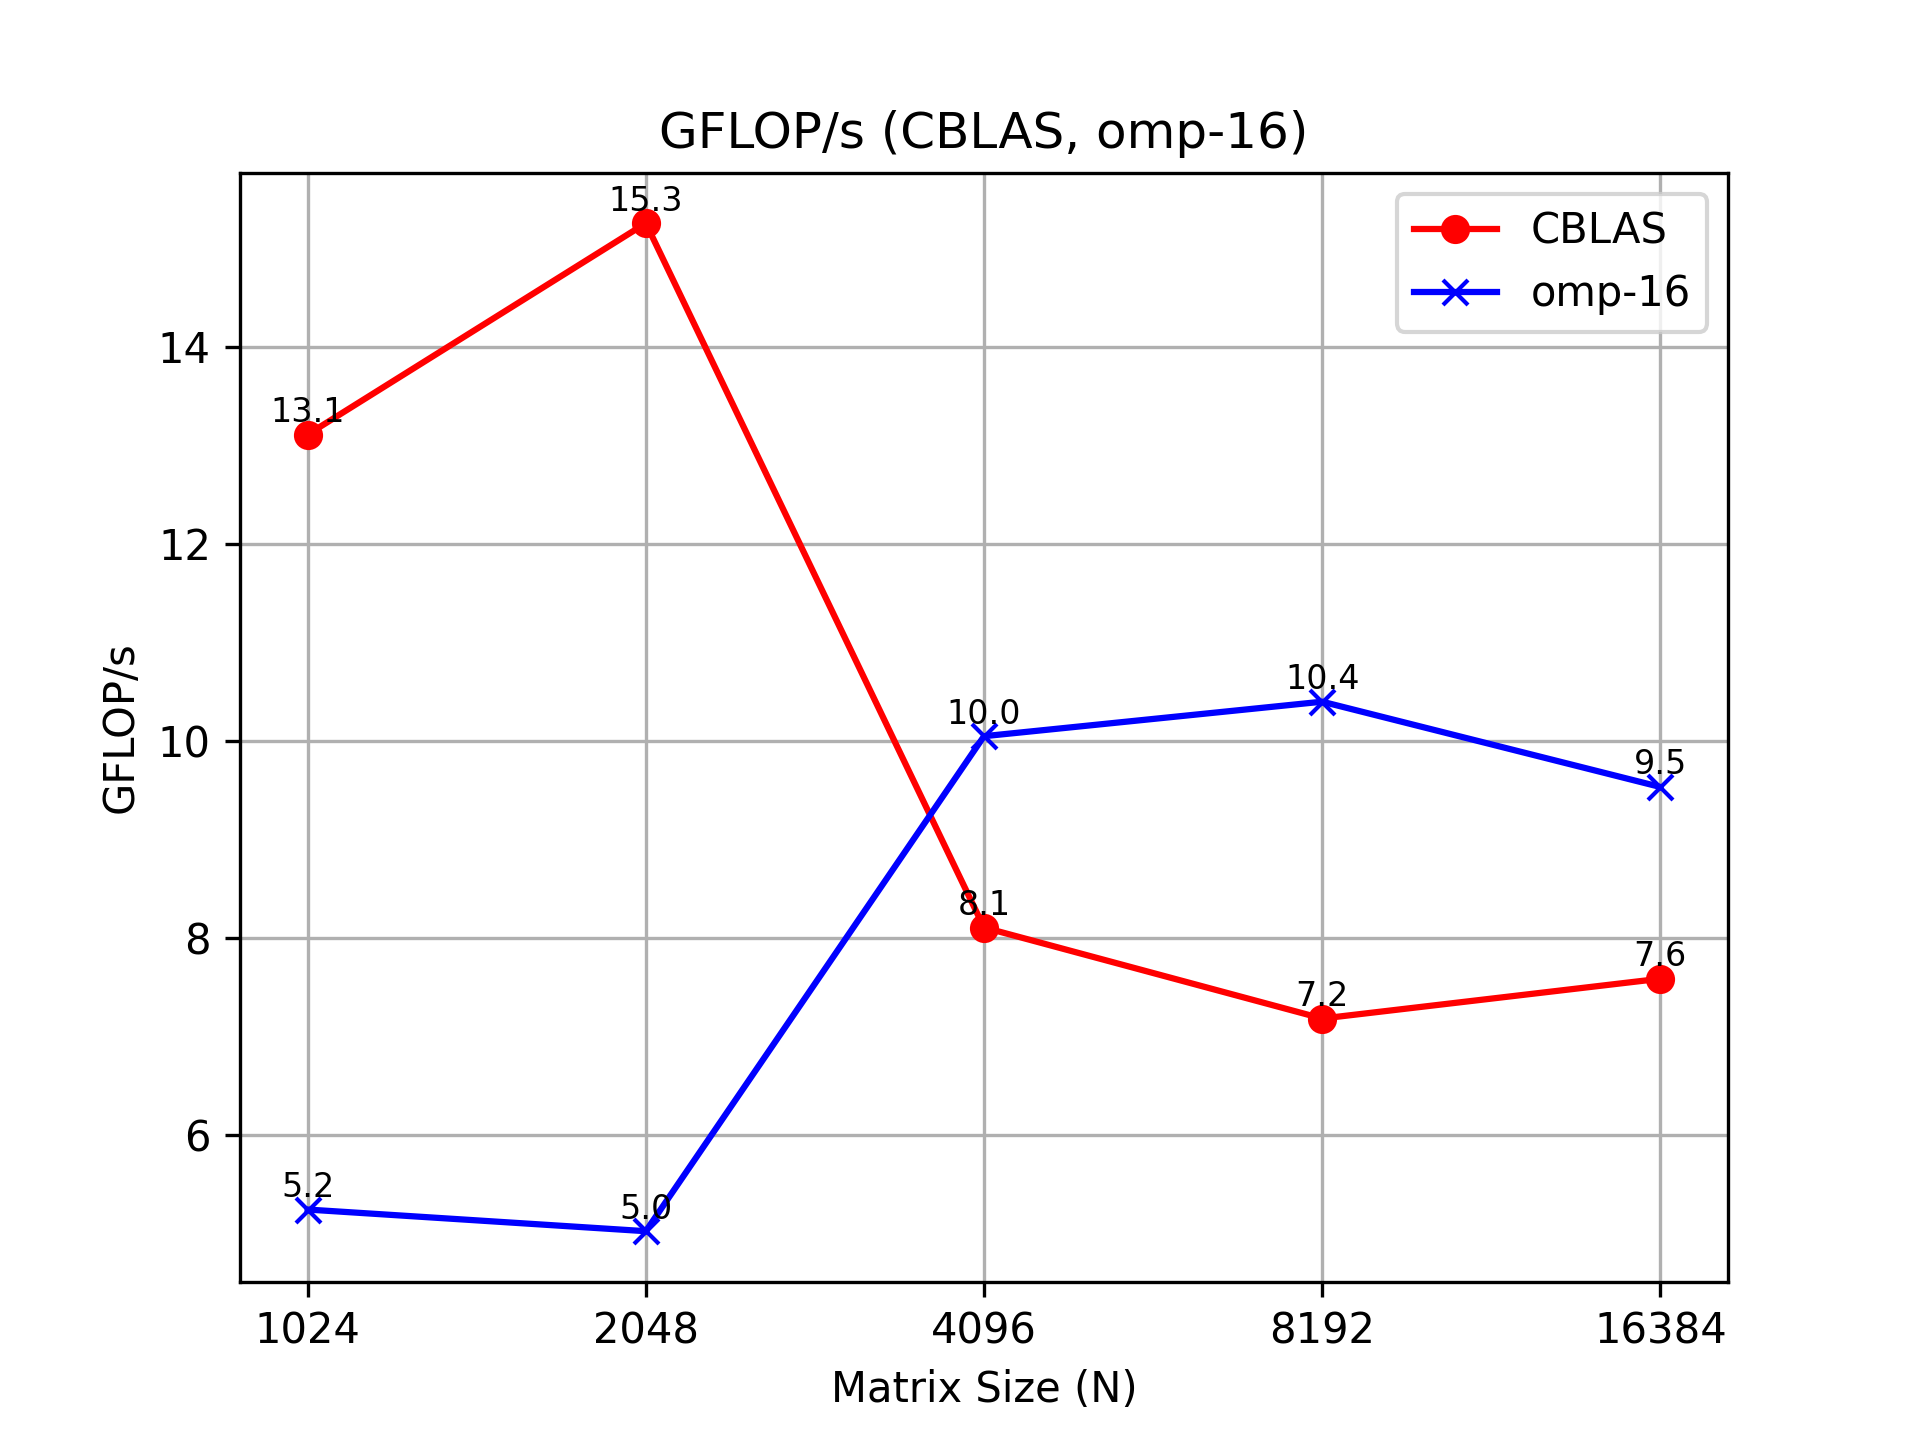
\includegraphics[width=1.0\linewidth]{images/GFLOPs-parallel.png}
    \caption{\textbf{Comparison of MFLOP/s between VMM OpenMP (omp-16) and VMM CBLAS across different matrix sizes.} The figure shows that for smaller matrix sizes (N=1K, 2K), CBLAS significantly outperforms omp-16, likely due to better cache optimization and lower threading overhead. For larger matrix sizes (N=4K, 8K, 16K), omp-16 outperforms CBLAS, benefiting from parallelism when the data no longer fits in the cache.}
    \label{fig:gflops-parallel}
\end{figure}

\subsection{Overall Findings and Discussion}
\label{subsec:overall-findings-and-discussion}
% \begin{itemize}
%     \item Memory bandwidth \% utilization across various implementations. Prepare a Table where the rows are different problem sizes, the columns are different implementations (CBLAS, basic, omp-1, omp-4, omp-16, omp-64), and entries are \% of peak bandwidth utilization. Discuss the following points/ideas:
%     \begin{itemize}
%         \item Which configuration has the best \% bandwidth utilization, and why?
%         \item Which configuration has the worst \% bandwidth utilization, and why?
%         \item For the OpenMP runs, how does \% bandwidth utilization change as a function of level of concurrency?
%     \end{itemize}
%     \item Parallel performance and scalability. Considering the data in your charts, is your implementation exhibiting linear speedup? That is, if the time required to do a problem size of N using 1 thread is T, then a true linear speedup using P threads would be T/P for the same problem size N. Discuss why or why not.
% \end{itemize}

The analysis of memory bandwidth utilization across different configurations reveals several insights. For the smallest matrix size (N=1K), CBLAS demonstrates the highest utilization, showing that it efficiently uses available memory resources when the problem fits well in the cache. On the other hand, the basic implementation for the largest matrix size (N=16K) shows the worst memory bandwidth utilization, indicating poor scalability and limited optimization in handling larger data.

Interestingly, the expectation that higher thread counts would yield better bandwidth utilization was not entirely met. For smaller matrix sizes, a single-threaded implementation (omp-1) performed best, likely due to lower overhead and more efficient use of cache. For larger matrix sizes (N=4K, 8K, 16K), the utilization for omp-4, omp-16, and omp-64 was similar, with omp-4 showing slightly better results. This can be explained by the data being confined to a single NUMA node, preventing full utilization of all 8 NUMA nodes. To maximize memory bandwidth, data needs to be distributed across all NUMA nodes, allowing concurrent access from each local NUMA node.

The calculation of memory accesses includes redundant access to vector \(x\), which occurs \(n\) times. If two rows of the matrix fit into the cache, effective utilization of the cache can reduce the memory accesses by approximately half. The high bandwidth utilization observed for CBLAS, reaching around 100 GB/s, is likely due to this optimization, effectively reducing the number of memory accesses. In practice, this suggests that CBLAS utilizes about 50 GB/s of memory bandwidth, which aligns with the theoretical limit of a single NUMA node's bandwidth. Given that the CPU has a peak memory bandwidth of 204.8 GB/s with 4 NUMA nodes, a single NUMA node can effectively provide about a quarter of this bandwidth, or roughly 51 GB/s, matching our observations.

In terms of scalability, we initially expected a nearly ideal speedup for larger matrix sizes, with omp-4 achieving 4x, omp-16 achieving 16x, and omp-64 achieving 64x speedup. However, the actual results showed significant bottlenecks, primarily due to limited memory bandwidth and inefficient memory allocation across NUMA nodes. The lack of memory distribution across NUMA nodes meant that the available bandwidth was restricted, leading to lower-than-expected speedups. Additionally, adding more threads, as in the case of omp-64, introduced additional overhead without resolving the bottleneck, which explains why omp-16 performed slightly better for larger problem sizes.

% Table for GB/s
\begin{table}[h!]
\centering
\begin{tabular}{|c|c|c|c|c|c|}
\hline
\multirow{2}{*}{Method} & \multicolumn{5}{c|}{Matrix Size N (GB/s)} \\ \cline{2-6} 
                        & 1K      & 2K      & 4K      & 8K      & 16K     \\ \hline
CBLAS                   & 104.96  & 122.08  & 64.86   & 57.46   & 60.68   \\ \hline
Basic                   & 18.87   & 18.86   & 18.48   & 18.47   & 18.39   \\ \hline
Vectorized              & 79.97   & 72.98   & 65.33   & 63.58   & 62.33   \\ \hline
omp-1                   & 73.02   & 61.04   & 53.81   & 54.62   & 53.50   \\ \hline
omp-4                   & 40.96   & 43.88   & 86.89   & 80.50   & 76.55   \\ \hline
omp-16                  & 41.98   & 40.20   & 80.39   & 83.18   & 76.25   \\ \hline
omp-64                  & 22.69   & 37.72   & 79.67   & 80.56   & 74.00   \\ \hline
\end{tabular}
\caption{\textbf{Memory bandwidth in GB/s for varying matrix sizes.} The matrix is \(N \times N\). The table shows how different implementations use available memory bandwidth across varying matrix sizes. CBLAS exhibits high utilization for smaller matrices, while OpenMP implementations show improved utilization for larger matrices due to increased concurrency.}
\label{tab:memory-bandwidth-gbps}
\end{table}

% Table for Percentages
\begin{table}[h!]
\centering
\begin{tabular}{|c|c|c|c|c|c|}
\hline
\multirow{2}{*}{Method} & \multicolumn{5}{c|}{Matrix Size N (\% Peak)} \\ \cline{2-6} 
                        & 1K      & 2K      & 4K      & 8K      & 16K     \\ \hline
CBLAS                   & 25.6\%  & 29.8\%  & 15.9\%  & 14.0\%  & 14.8\%  \\ \hline
Basic                   & 4.6\%   & 4.6\%   & 4.5\%   & 4.5\%   & 4.5\%   \\ \hline
Vectorized              & 19.5\%  & 17.8\%  & 16.0\%  & 15.5\%  & 15.2\%  \\ \hline
omp-1                   & 17.9\%  & 14.9\%  & 13.2\%  & 13.4\%  & 13.1\%  \\ \hline
omp-4                   & 10.0\%  & 10.7\%  & 21.2\%  & 19.7\%  & 18.7\%  \\ \hline
omp-16                  & 10.2\%  & 9.8\%   & 19.7\%  & 20.3\%  & 18.6\%  \\ \hline
omp-64                  & 5.6\%   & 9.2\%   & 19.5\%  & 19.7\%  & 18.1\%  \\ \hline
\end{tabular}
\caption{\textbf{Memory bandwidth utilization (\%) for varying matrix sizes.} The matrix is \(N \times N\). The table illustrates the percentage of peak memory bandwidth utilization for each implementation. CBLAS achieves high utilization for small matrices, while OpenMP implementations make better use of available bandwidth as matrix size increases, albeit with diminishing returns for higher thread counts.}
\label{tab:memory-bandwidth-utilizatoin-percentage}
\end{table}